\documentclass[a4 122pt]{article}

\usepackage{color}
\usepackage{polski}
\usepackage[utf8]{inputenc}
\usepackage{amsmath}
\usepackage{amsthm}
\usepackage{todonotes}
\usepackage{geometry}
\usepackage{hyperref}
\geometry{
  body={6.5in, 8.5in},
  left=0.7in,
  top=0.45in,
  bottom=0.3in
}
\usepackage{graphicx} % załączanie obrazów

\title{Planarność grafu}
\author{Paweł Sokołowski\\Michał Kaszlej}


\begin{document}


\maketitle

	\section{Cel projektu}

		Celem projektu jest napisanie algorytmu heurystycznego sprawdzającego czy zadany graf jest planarny.
		Według twierdzenia podanego w książce (Wilson, 1998):

		\begin{figure}[h]
			\begin{center}
				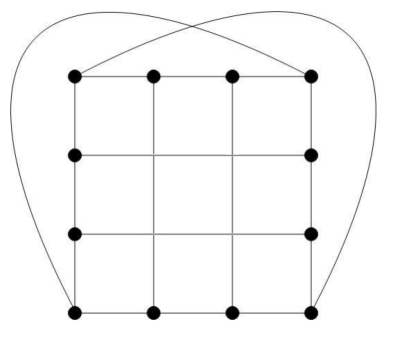
\includegraphics[width=0.5\textwidth]{include/graf.png}
				\caption{Zadany graf}
			\end{center}
		\end{figure}


		Dany graf jest planarny wtedy i tylko wtedy, gdy nie zawiera podgrafu ściągalnego do grafu $K_{3.3}$ lub do grafu $ K_5 $

	\section{Język programowania} 

		Algorytm zostanie zaimplementowany za pomocą języka C\#.

	\section{Algorytm}

		Algorytm rozwiązujący zadany problem zostanie wybrany w dalszej fazie projektu.

	\section{Bibliografia}

		Wilson, R. J. (1998). Wprowadzenie do teorii grafów. Warszawa: Wydawnictwo Naukowe PWN.

\end{document}	
